\section{Durchführung}
\label{sec:Durchfuehrung}
In diesem Kapitel sollen die einzelnen Schritte des Versuches erklärt werden.\\

Zunächst wird mittels einer Hall-Sonde die Magnetflussstärke des verwendeten Elektromagneten vermessen, um den Zusammenhang zwischen der Flussstärke und der eingestellten Stromstärke berechnen zu können.\\
Danach wird der Versuch wie in \autoref{fig:vaufbau} aufgebaut.
Das aus der Spektrallampe tretende Licht wird auf ein Geradsichtprisma fokussiert.
Dieses lenkt das Licht wellenlängenabhängig ab.
Ein eingebrachter Polarisationsfilter lässt danach die verschiedenen Übergänge voneinander trennen.
Der Spalt $S_2$ lässt je nach Einstellung nur einen kleinen Wellenlängenbereich, um die zu untersuchende Wellenlänge hindurch.
Zuletzt wird das Licht durch eine Linse auf die Lummer-Gehrcke Platte geleitet und danach mittels einer Kamera photographiert.

\begin{figure}
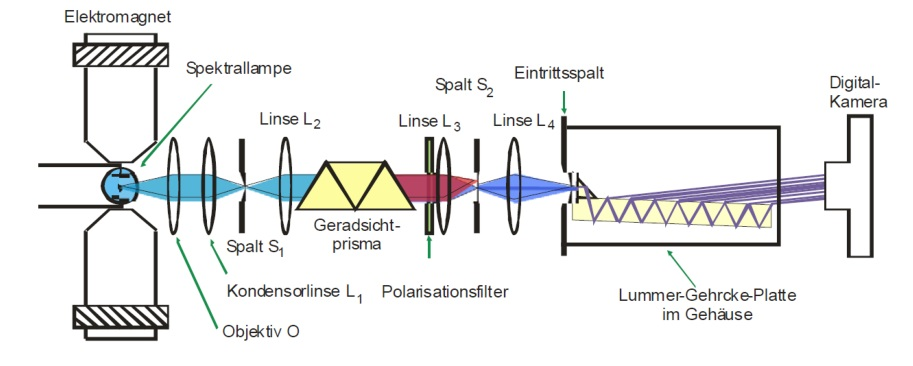
\includegraphics{content/grafiken/Aufbau.jpg}
\caption{Versuchsaufbau}
\label{fig:vaufbau}
\end{figure}

Untersucht wurde die Aufspaltung der Spektrallinien bei 480\,nm und 643,8\,nm Wellenlänge. Dazu wurde jeweils vier Photos gemacht.
Zwei Photos mit eingeschaltetem Magnetfeld für parallel zum Magnetfeld und senkrecht dazu polarisierte Strahlung und zwei Photos ohne Magnetfeld für dieselben Polarisationen.
